\documentclass{beamer}


\usepackage[utf8]{inputenc}
\usepackage{pgfpages}
\usepackage{xcolor}

\setbeameroption{show notes}
\setbeamertemplate{note page}[plain]
\setbeameroption{show notes on second screen=left}

\usetheme{Warsaw}
\graphicspath{ {./images/}{../images/}{../kcov-swedencpp/images/}{../../kcov-swedencpp/images/}{output/} }

\AtBeginSection[specialframe]
{
  \begin{frame}{Table of Contents}
   \tableofcontents[currentsection]
  \end{frame}
}

\title[What's in a binary?] %optional
{What's in a binary?}

%\subtitle{A short story}

\author{Simon Kågström}

\institute
{
  Consultant\\
  \texttt{https://github.com/SimonKagstrom/emilpro}
}

%\logo{\includegraphics[height=1.5cm]{lion-logo.png}}

\begin{document}

\begin{frame}
  \titlepage
  \note{My name is Simon Kågström and I work as a consultant, currently at Profoto. Tonight I will present emilpro.

So let's get started!}
\end{frame}


\begin{frame}{Background}
  \begin{itemize}
    \item I have a few themes that I often return to in my projects
    \item During the years, I've multiple times had to rely on disassembly for debugging
    \item Objdump output is cumbersome to navigate through
    \item<2> I wanted a graphical application that allows easier navigation
  \end{itemize}
\end{frame}


\begin{frame}
  \frametitle{Demo}
  \note<1->{
    \footnotesize
  }

  \note<2>{
  }
  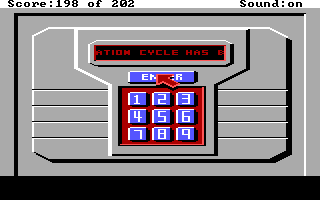
\includegraphics[width=\linewidth]{sq_keypad}
  % Start the app. Show symbols, cross-reference, 
  %\includegraphics<1>[height=8cm]{goto_fail_no_coverage}
  %\includegraphics<2>[height=8cm]{goto_fail}
\end{frame}

\begin{frame}{Binary formats}
  \begin{itemize}
    \item \textbf{Linux/FreeBSD} etc: ELF
    \item \textbf{MacOS}: Mach-O
    \item \textbf{Windows}: PE
  \end{itemize}
    % ELF + DWARF
    % Mach-O
    % PE
    % The three rules for an instruction set architect
    \note{
      The binary format is used for executables and linkable object files. These are the
      three main formats used today.

      The job description for an instruction set architect
      \begin{itemize}
        \item You should create an instruction set which consists of abbreviations of
        common words for no particular reason. Bonus point for using unclear meanings
        (for example MOV, which is an abbreviation of "move", but actually copies the
        value)
        \item Your instruction set should be basically MIPS, but with a few improvements.
        Sometimes "improvements".
        \item Your instruction set should contain at least one funny sounding instruction.
        Case in point: EIEIO.
      \end{itemize}
    }

    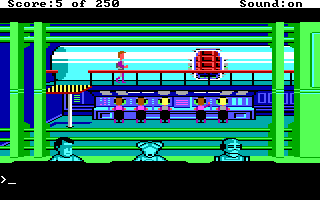
\includegraphics[width=7cm]{sq2_computer_room}
  \end{frame}

  \begin{frame}{Actors and objects}
    Actors
    \begin{itemize}
      \item \textbf{Compiler}
      \item \textbf{Linker}
      \item \textbf{Loader}
      \item \textbf{Disassembler}
    \end{itemize}
    Objects
    \begin{itemize}
      \item \textbf{Sections}: Text, data, debug info etc
      \item \textbf{Symbols}: Functions/methods, variables, ...
      \item \textbf{Relocations}: 
    \end{itemize}
    % What is compiler, linker, loader?
    % Show in emilpro

    % Sections, symbols, relocations
    % Disassembler, compiler, linker, loader
\end{frame}

\begin{frame}{Relocations}
  \begin{itemize}
    \item ...
  \end{itemize}
\end{frame}

\begin{frame}{Producing a binary}
  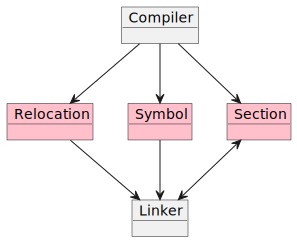
\includegraphics[width=7cm]{compiler_linker}
\end{frame}

\begin{frame}{Loading a binary}
  Different categories of binaries are handled differently:
  \begin{itemize}
    \item Execute from direct-mapped flash (embedded systems)
    \item Static executables
    \item Dynamic executables
    \item PIEs (Position-Independent Executables)
  \end{itemize}

  % Sections, symbols, relocations
  % Example from embedded system
  % Load sections into memory
  % Entry point
  % Disassembler, compiler, linker, loader
  \includegraphics[width=7cm]{loader}
\end{frame}

\begin{frame}{PIEs}
    % Relocation entries
    % Why are they needed?
\end{frame}

\begin{frame}{How to write a dissassembler?}
    %libbfd
    %capstone
    %qt
    % Newton: "If I hadn't been standing on the shoulders of giants, I wouldn't have reached the apple."
    \includegraphics[width=7cm]{disassembler}
\end{frame}

\begin{frame}{libbfd}
    %Example from documentation
\end{frame}

\begin{frame}{Implementation}
    %PlantUML
    Span, span span
    \includegraphics<2>[height=4cm]{spam}
\end{frame}

\begin{frame}{Why is this easier now than 10 years ago?}
    %conan
    %c++11+
    %copilot
    %move from binutils
\end{frame}




\begin{frame}{Questions and comments!}
  \footnotesize
  (Images from \url{http://www.falselogic.net/LetsPlay/SpaceQuest.html})
  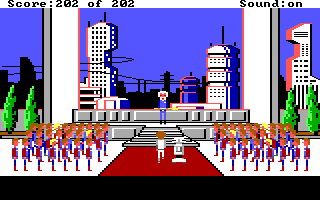
\includegraphics[width=\linewidth]{sq_final}
\end{frame}

\end{document}
